% CAPITULO 4-------------------------------------------------------------------

\chapter{TAREFA 4: DESENVOLVIMENTO MOBILE}
\label{sec:tarefa4}

O desenvolvimento mobile é um dos nichos que mais crescem no mercado da tecnologia.

Dentro das corporações, a tecnologia mobile proporciona uma série de benefícios, entre eles o acesso mais rápido e prático às informações — o que facilita a análise de dados, o gerenciamento e a tomada de decisão.

\section{O que é a Tecnologia Mobile}

A tecnologia \textit{mobile} é aquela que permite a movimentação do usuário durante o seu uso.

No meio corporativo, essa mobilidade possibilita uma gestão mais assertiva sobre os negócios uma vez que permite ao usuário administrar a empresa a qualquer hora e em qualquer lugar.

Então, o desenvolvimento mobile está relacionado a criação dessa tecnologia.

Por ser cada vez mais importante no dia a dia de pessoas e empresas, a tecnologia mobile deixou de ser vista apenas como um recurso e passou a ser uma necessidade.

Hoje é possível integrar o \textit{desktop} ao celular, de forma inovadora, e assim aumentar a produtividade e oferecer uma experiência personalizada para o cliente.

\section{A Importância do Desenvolvimento de Software Móvel}

A popularização dos \textit{smartphones} tem contribuído para mais pessoas utilizarem dispositivos móveis.

Como a tendência é que os usuários se tornem cada vez mais mobile e as empresas recorram a tecnologia para otimizar funções, caberá aos desenvolvedores criar apps capazes de atender essa demanda.

Não só para otimizar tarefas e ajudar na gestão corporativa, o desenvolvimento de \textit{software} móvel também é importante para manter o cliente um passo à frente da concorrência.

\section{Linguagens de Programação para Desenvolvimento Android}

Muitas empresas têm feito dos aplicativos o seu principal negócio e meio de comunicação com o cliente. Mas quais são as habilidades necessárias para se desenvolver um aplicativo Android do zero? Há algumas linguagens de programação que são mais indicadas do que outras para a tarefa, ao mesmo tempo, vale lembrar que é preciso um roteiro bem estruturado para não cometer os erros mais comuns ao desenvolvê-lo.

\section{Como funciona o sistema Android}

O Sistema operacional Android, criado pela Android Inc em 2003 e adquirida pela Google em 2005, usa um típico Kernel Linux.

Este Kernel conta com algumas modificações, principalmente quando se trata de gerenciamento agressivo de memória, consumo de energia e outras melhorias específicas para dispositivos móveis.

Todas as linguagens de programação para Android contam com, ao menos, um de dois kits de desenvolvimento. O primeiro é o NDK (Kit de Desenvolvimento Nativo).

Este pode ser manipulado utilizando C/C++ ou Java.

O segundo kit de desenvolvimento é o Android SDK (Kit de Desenvolvimento de Software ou DevKit).

Trata-se de uma plataforma de mais alto nível, responsável pelo ecossistema de desenvolvimento da plataforma.

O Android SDK inclui projetos de exemplo com código fonte, ferramentas de desenvolvimento, emulador e outras bibliotecas que auxilia os desenvolvedores a utilizarem a plataforma.

Antes de continar, precisamos definir as duas formas possiveis de desenvolvimento: desenvolvimento nativo e desenvolvimento híbrido.

\section{Desenvolvimento Nativo}

Em desenvolvimento nativo, é necessário um especialista na linguagem específica daquela plataforma que se deseja gerar um aplicativo, seja Android ou iOS.

Também possui acesso à todos os recursos do dispositivo, com bom desempenho (acelerômetro, giroscópio, geolocalização, etc), como são desenvolvidos especificamente para cada plataforma, explora muito bem toda a UI.

\section{Desenvolvimento Híbrido}

Já em desenvolvimento híbrido, não é necessário um especialista em linguagem nativa, muitas vezes utiliza-se linguagens que não são específicas daquela plataforma, e com um único código fonte, pode-se gerar aplicativos para plataformas diferentes (Android e IOS).

Respeita-se a UI do sistema operacional do dispositivo, porém, utiliza um navegador embutido no aplicativo para demonstrar ao usuário.

Cada uma dessas modalidades tem seu espaço no mercado, basicamente esse pode ser considerado mais um indicador, busque também por vagas em mobile, só que levando em conta que produto te agradaria mais trabalhar.

\section{Linguagens de Programação para Android}

\subsection{Java}

\begin{figure}[H]
    \centering
    
\includegraphics[width=0.3\linewidth]{dados/figuras/java}
    \caption{Java}
    \label{fig:java}
\end{figure}

É uma linguagem que utiliza o paradigma Orientado a Objetos, e mais recente, tem trabalhado forte em inserir elementos de programação Funcional em seu escopo.

É tido como a linguagem oficial para o desenvolvimento do Android e é suportado pelo Android Studio.

\textbf{Pontos positivos do Java}

\begin{itemize}
    \item Muitos tutoriais e dicas na internet sobre a mais variada gama de assuntos da linguagem;
    \item Uma das linguagens mais mais usadas para fazer aplicativos Android;
    \item Suporta Android Studio;
    \item É versátil.
\end{itemize}

\textbf{Pontos negativos do Java}

\begin{itemize}
    \item Curva de aprendizado é bastante íngreme;
    \item Sobrecarga de conteúdo pode mais atrapalhar que ajudar se você não sabe o que procura;
    \item Não é a linguagem de computador mais amistosa para leitura;
    \item Atualizações frequentes dificultando o processo das atualizações.
\end{itemize}

\subsection{LUA (Corona SDK)}

\begin{figure}[H]
    \centering
    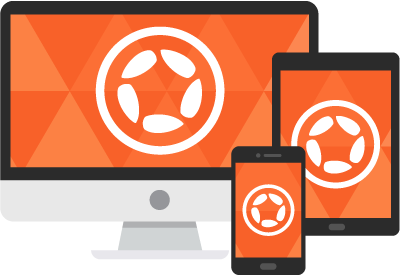
\includegraphics[width=0.3\linewidth]{dados/figuras/corona}
    \caption{LUA (Corona SDK)}
    \label{fig:corona}
\end{figure}

Esta é uma das opções mais simples para quem quer desenvolver aplicações para Android.

Estamos falando da linguagem de \textit{scripting} Lua, poderosa e fácil de aprender, com Corona SDK.

Caso não conheça, Corona é um \textit{framework} que lhe deixa criar jogos e aplicativos para \textit{mobile}, desktop, TVs e tudo mais que rode Android.

Existem alguns benefícios em usar o Corona SDK para desenvolver aplicativos Android. Os devs por trás da Corona dizem que seu produto permite que os desenvolvedores trabalhem em aplicativos móveis com uma velocidade dez vezes maior.

\textbf{Pontos positivos de usar LUA com Corona SDK}

\begin{itemize}
    \item Simples, fácil de aprender e poderoso;
    \item É uma linguagem de programação muito rápida de usar;
    \item Suporte para todas as bibliotecas nativas, podendo publicar em várias plataformas;
    \item Emulador que permite ver sem compilar o código;
\end{itemize}

\textbf{Pontos negativos de usar LUA com Corona SDK}

\begin{itemize}
    \item Precisa de um editor para o código;
    \item É limitado em comparação com outras linguagens;
    \item Exige pagamento para a utilização de alguns recursos.
\end{itemize}

\subsection{Kotlin}

\begin{figure}[H]
    \centering
    
\includegraphics[width=0.3\linewidth]{dados/figuras/kotlin}
    \caption{Kotlin}
    \label{fig:kotlin}
\end{figure}

Kotlin é uma linguagem de programação reconhecida pela Google que pode ser usada como alternativa ao Java para desenvolvimento de aplicativos Android. E geralmente é isso mesmo que ocorre.

Ele pode interoperar com Java e é executado na Java Virtual Machine.

\textbf{Pontos positivos do Kotlin}

\begin{itemize}
    \item Suporte a Java Virtual Machine;
    \item Não faz com que o tamanho dos arquivos aumente;
    \item Não causa desaceleração;
    \item É simplificado;
    \item Ideal para começar com Android;
    \item Suporta Android Studio.
\end{itemize}

\textbf{Pontos negativos do Kotlin}

\begin{itemize}
    \item Embora seja fácil de aprender, não é tão fácil quanto outras linguagens citadas;
    \item O suporte da comunidade é bem menor, por não ser tão popular.
\end{itemize}

\subsection{C\#}

\begin{figure}[H]
    \centering
    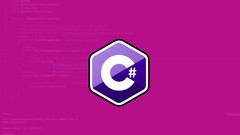
\includegraphics[width=0.3\linewidth]{dados/figuras/c}
    \caption{C\#}
    \label{fig:c}
\end{figure}

C\# é bastante semelhante ao Java e por isso é indicado para o desenvolvimento de aplicativos Android.

Outro motivo para aprender C\# se dá pelo fato de que hoje é a uma das mais importantes linguagens do mercado \textit{entreprise}.

É também uma linguagem Orientada a Objetos, mas com uma sintaxe mais simples do que Java, o que torna a codificação aparentemente mais fácil.

\textbf{Pontos positivos do C\#}

\begin{itemize}
    \item Simples de programar;
    \item Fácil de ler e entender;
    \item Orientado a objetos;
    \item Similar ao C++;
    \item Sem problemas de memória graças à coleta de lixo;
\end{itemize}

\textbf{Pontos negativos do C\#}
\begin{itemize}
    \item C\# e \textit{Unity} são excelentes para jogos 3D, mas não tão bons para desenvolver aplicativos padrão juntos;
    \item Não está de acordo com a linguagem do Material Design do Google;
    \item Existe menos liquidez no mercado para desenvolvedores profissionais de Android em C\#.
\end{itemize}

\subsection{JavaScript + CSS + HTML (PhoneGap)}

\begin{figure}[H]
    \centering
    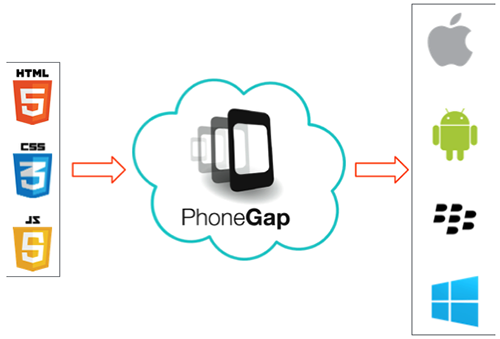
\includegraphics[width=0.3\linewidth]{dados/figuras/phonegap}
    \caption{JavaScript + CSS + HTML (PhoneGap)}
    \label{fig:phonegap}
\end{figure}

Os aplicativos Android também podem ser criados com HTML, CSS e JavaScript usando Adobe PhoneGap no Apache Cordova.

O framework PhoneGap permite criar aplicativos híbridos que são mostrados por meio do “WebView”, mas empacotados como um aplicativo.

A estrutura do PhoneGap dificilmente requer muita programação, exceto para JavaScript.

O PhoneGap, basicamente como o nome sugere, apenas preenche uma lacuna, dando aos desenvolvedores de aplicativos Android acesso a recursos do telefone, como a câmera ou o acelerômetro.

\textbf{Pontos positivos do JavaScript + CSS + HTML com PhoneGap}

\begin{itemize}
    \item Permite aos designers, front-ends ou qualquer pessoa que crie sites interativos usando HTML, JavaScript e CSS usar recursos mais simples do Android;
    \item Pode ‘quebrar um galho em situações’ bem específicas.
\end{itemize}

\textbf{Pontos negativos do JavaScript + CSS + HTML com PhoneGap}

\begin{itemize}
    \item Para tarefas básicas, ele dará conta, mas não para a maior parte das funções;
    \item Esta opção não está presente no ‘cinto de utilidades’ do desenvolvedor Android profissional.
\end{itemize}

\section{Tendências no Desenvolvimento Móvel}

Acompanhar todas as tendências também pode ser um desafio. Afinal, a tecnologia passa por mudanças constantes e toda essa oscilação vai exigir conhecimento para a software house não correr o risco de levar um produto ultrapassado para o cliente.

Para se manter atualizado, veja agora algumas tendências no desenvolvimento mobile:

\subsection{Inteligência artificial e aprendizado da máquina}

Oferecer funcionalidades inteligentes é o que vai agregar valor a sua solução mobile. Portanto, investir em inteligência artificial e aprendizado da máquina é importante para deixar o seu produto mais moderno e valorizado em relação ao dos concorrentes

\subsection{Integração com IoT e Dispositivos (\textit{wearables})}

\textit{Wearables} são dispositivos que podem ser “vestidos” ou integrados ao corpo do usuário (relógios inteligentes, pulseiras e óculos de realidade virtual).

O sucesso dessa tecnologia está atrelado à integração do sistema operacional com a Internet das coisas, que permite o gerenciamento de diversos objetos digitais.

\subsection{Application Performance Measurement (APM)}

\textit{Application Performance Measurement} está relacionado ao monitoramento e gestão de desempenho e disponibilidade de aplicativos. Se o desenvolvedor não fizer esse gerenciamento, ele não consegue garantir a disponibilidade e nem a qualidade do \textit{software}.

\subsection{Enterprise Mobile Management (EMM)}

\textit{Enterprise Mobile Management}é o gerenciamento de mobilidade corporativa. À medida que mais empresas compram dispositivos e buscam suporte para o uso dessas ferramentas, o EMM se torna cada vez mais necessário.

\subsection{Realidade Aumentada}

Realidade aumentada está relacionada à integração de elementos ou informações virtuais ao dispositivo móvel. Essa tecnologia oferece experiências mais ricas ao usuário uma vez que é usada para otimizar ambientes ou situações do cotidiano.

\subsection{Gateway de Pagamentos}

\textit{Gateway} de pagamento é um serviço destinado a empresas de grande porte, lojas virtuais e sistemas SaaS. No dispositivo, uma operadora financeira é responsável por autorizar pagamentos de transações online em \textit{websites} de empresas ou pessoas físicas.


\nocite{geek}
\nocite{css3}
\nocite{devweb}
\nocite{queconceito}
\nocite{metodologia}
